\section{Softwarearchitektur des Radarsimulators}

Im folgenden Abschnitt werden die einzelnen Softwarekomponenten der Radarsimulator Anwendung beschrieben und auf Wiederverwendbarkeit und Modularität überprüft. Dabei wird sich auf die Kernkomponenten der Anwendung beschränkt. Diese sind die SimulatorInstance, die View-Komponente und das Datenmodell. Der Radarsimulator wird von Thales zur Verfügung gestellt und wurde, vor und während dem Schreiben des Kapitels, nicht verändert. Der Radarsimulator mit neuer Architektur wird als Testsimulator bezeichnet.

Der Radarsimulator ist eine Eclipse RCP Anwendung und setzt sich aus mehreren Equinox Plug-In Modulen zusammen. Er wird durch Basis- und weiteren
Plug-Ins der Venus unterstütz. Diese stellen spezifische Funktionen, wie Anwendungsstruktur und Helferklassen zur Verfügung.Der Startpunkt der Anwendung 
ist die Klasse SimulatorMain, welche sich in dem Modul RadarSimulator.app befindet. Dieses Modul stellt die Benutzeroberfläche des Simulators zur 
Verfügung. Im Modul werden die Startklasse der Anwendung und weitere Fenstereinstellungen für diese Anwendungen in einer Applikation.e4xmi-Datei 
angegeben. Diese Datei ist die Basis jeder Eclipse RCP Applikation. Wenn die Eclipse Applikation die Startklasse in Java aufruft, startet der 
RestartService. Diese ist im folgenden Codeabschnitt zu sehen.

\begin{lstlisting}

public double getAzimuthStepSize() {
	return azimuthStepSize;
}

public boolean isClockwise() {
	return clockwise;
}

\end{lstlisting}

Die gesamte Funktionalität der Sensorsimulation stellt die SimulatorInstance zur Verfügung. Wenn der RestartService die SimulatorInstance erfolgreich geladen hat, initialisiert dieser die Benutzeroberfläche der Anwendung. Außerdem ermöglicht es der RestartService, die Simulation durch einen Mausklick in ein Fenster Menü item neu zu starten. Dabei werden die Benutzeroberfläche, sowie die SimulatorInstance neu geladen. Der RestartService soll zudem auch im zukünftigen Testsimulator sowie im Trainer- und Traineesimulator enthalten sein. Die SimulatorInstance und der SimulatorMainContentProvider werden in der SimulatorMain als Attribute gespeichert. Wenn die Benutzeroberfläche geladen wird, bekommt diese die SimulatorInstance übergeben, damit diese die Simulation steuern kann. Wie es bei einer Eclipse Applikation üblich ist sind Funktionen der Anwendung in Softwaremodule eingeteilt. Diese Module heißen bei Eclipse Plug-Ins. In der folgenden Abbildung erkennt man die Aufteilung der Hauptkomponenten in zwei Plug-Ins.

\begin{figure}[h!]
    \centering
    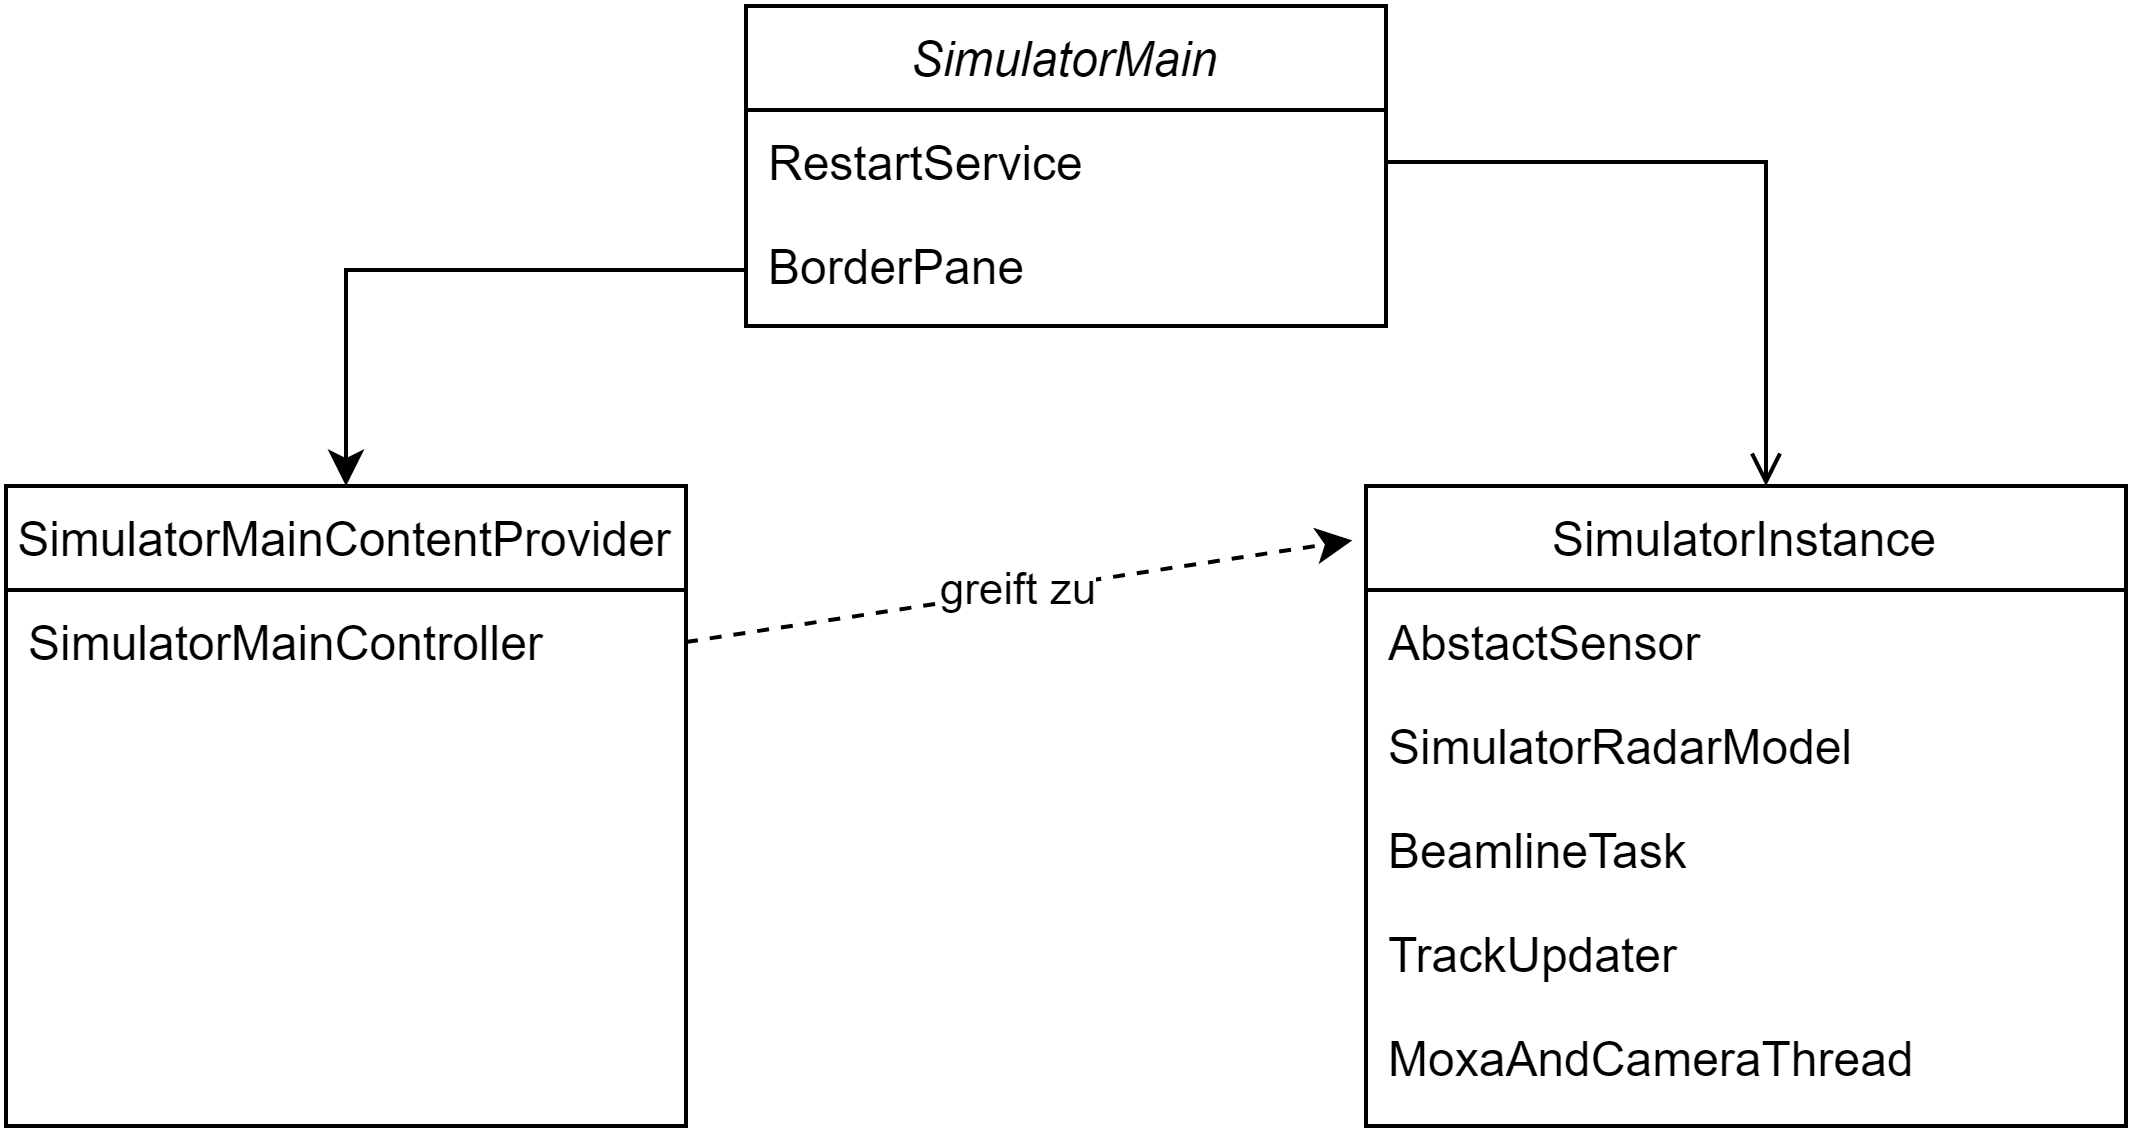
\includegraphics[width=0.8\textwidth]{content/assets/RadarSimulatorUML.png}
    \caption{UML-Diagramm des Radarsimulators}
\end{figure}

\input{content/Analyse/benutzeroberfläche}
\subsection{SimulatorInstance}
Die SimulatorInstance hat folgende Aufgaben:
\begin{itemize}
    \item Erstellen des Datenmodells des Simulators. Aufgrund von unterschiedlichen Werten und Zubehör zwischen den Sensortypen, wird das Datenmodell je nach Sensortyp und Asterix-version entsprechend befüllt. Dafür wird eine Helferklasse verwendet.
    \item Erstellen eines Sensors, je nach Sensortyp wird ein passender Sensor initialisiert. 
    Der AbstractSensor ist die Vaterklasse der jeweiligen Sensortypen (\texttt{SensorBORA}, SensorGO12, SensorGO80 und SensorGA10). Über den Sensor können \\Asterix-Kommandos an die Venus versendet werden
    \item Erstellen und starten des BeamlineTasks. Der BeamlineTask ist dafür zuständig, dass sich die Beamline des Sensors korrekt bewegt und die entsprechenden Werte im Modell geupdatet werden.
    \item Erstellen und starten des Trackupdater. Er ist dafür zuständig die Tracks korrekt upgedatet werden und über das Asterixinterface versendet werden.
    \item Erstellen und starten des MoaxaAndCameraServerTask. Dieser simuliert optionales Zubehör und die Kamera, falls dieser vorhanden ist.    
    
\end{itemize}

Diese Tasks haben eine klar definierte Aufgabe und lassen sich gut wiederverwenden.
\subsection{Model}


Das Datenmodell des Radarsimulators wird mithilfe des Frameworks EMF erstellt. Das Modell befindet sich in einem eigenen Plug-In Modul. Darin sind ein graphisches Entity-Relation-Diagramm des Modells und der daraus generierbare Modellcode enthalten. Das Objekt, welches die Informationen des Sensors zusammenfasst, heißt SimulatorModelRadar. Dieses enthält 19 Attribute, die die Eigenschaften des simulierten Sensors beschreiben. Zusätzlich gibt es noch Beziehungen zu zehn Klassen, die die Daten des Sensors speichern. 

Die Klassen, die in dieser Arbeit verwendet werden, sind:

\begin{itemize}
    \item SimulatorBitNode: Der SimulatorBitNode ist eine Baumdatenstruktur in der Bitfehler abgelegt werden. Das SimulatorModelRadar besitzt höchstens einen SimulatorBitNode.
    \item SimulatorModelEquipment: Der SimulatorModelRadar kann beliebig viele   \\
    SimulatorModelEquipment-Objekte des Sensors gespeichern. Weil die PNU ein Zubehör des Sensors ist, werden dessen Informationen als SimulatorModelEquipment gespeichert. Dafür gibt es eine Klasse, welche SimulatorModelEquipment erweitert. Diese heißt SimulatorModelPNU.
    \item SimulatorModelSector: Um Sektor Informationen des Sensors zu speichern, gibt es die Klasse SimulatorModelSector. Die Klasse SimulatorModelRadar hat höchstens einen aktuellen Sektor und beliebig viele weitere Sektoren.    
\end{itemize}

Was bei der Betrachtung des grafischen Modells auffällt ist, dass es drei vom SimulatorModelRadar unabhängige Klassen gibt. Diese Klassen sind:

\begin{itemize}
    \item \texttt{Scenario}: Die Klasse Scenario beinhaltet beliebig viele ScenarioTargets, welche beliebig viele Waypoints haben. Man erkennt daran gut wie das Scenario aufgebaut ist. Die ScenarioTargets sind mögliche Objekt, die der Sensor detektieren kann. Das sind zum Beispiel Fußgänger oder PKWs. Diese Objekte bewegen sich auf einem Pfad, welcher durch die Waypoints (auf Deutsch Wegpunkte) definiert wird.
    \item \texttt{TargetSimulation}:  Die TargetSimulation beschreibt die Eigenschaften, wie z.B. Position, Klassifizierung und Radarquerschnitt, eines Radarziels zu einem bestimmten Zeitpunkt. Eine TargetSimulation entsteht, wenn im UI ein Scenario abgespielt wird. Dabei wird die aktuelle Position eines ScenarioTargets, anhand der Wegpunkte berechnet und daraus wird eine TargetSimulation erstellt.
    \item SimulatorModelTrack: Ein SimulatorModelTrack beschreibt ebenso, wie die TargetSimulation, die Eigenschaften eines Radarziels. Der entscheidende Unterschied ist, dass dieses Radarziel nun abhängig vom Sensor ist. Deswegen hat dieser weitere Attribute, welche die Venus benötigt um das Ziel darzustellen. In Tabelle \ref{table:1} werden die entscheidenden Unterschiede der beiden Klassen aufgezeigt.    
\end{itemize}

\begin{table}[h]
    \begin{tabular}{ |c|c|c| } 
        \hline
         & \texttt{TargetSimulation} & \texttt{SimulatorModelTrack} \\ 
        \hline
        Koordinatensystem & Lat/Long & Polarkoordinaten \\ 
        \hline
        Doppler Speed Informationen & - & x \\ 
        \hline
        
   \end{tabular}
   \caption{Vergleich zwischen\texttt{TargetSimulation} und \texttt{SimulatorModelTrack}}
   \label{table:1}
\end{table}

Wie sinnvoll ist es nun diese Klassen vom Modell zu trennen? Das Scenario wird von der UI Komponente verwendet, um es auf einer Karte darzustellen und um es als XML-Datei zu speichern. Wie man in Abbildung \ref{figure:scenarioview} erkennen kann gehört das Scenario zum ScenarioController und lediglich der ScenarioUpdater ist vo ihm abhängig. Deswegen ist es nicht notwendig das Scenario im Modell zu speichern und es müssen keine Änderungen vorgenommen werden.

\begin{figure}[h!]
    \centering
    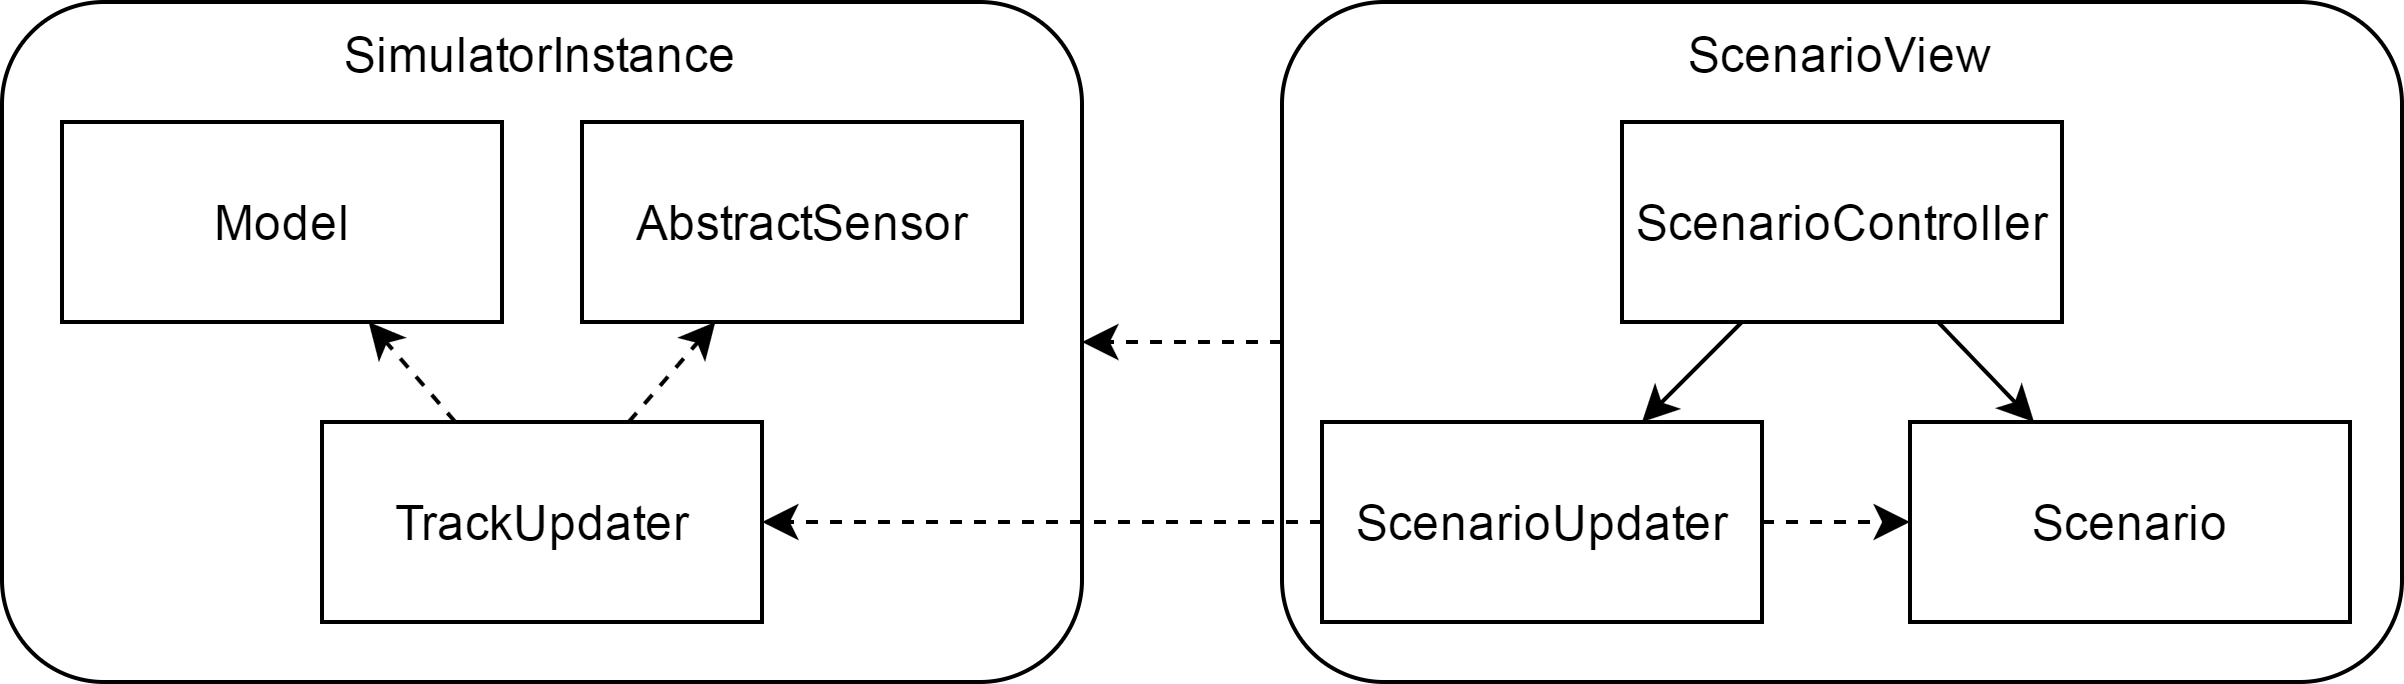
\includegraphics[width=1\textwidth]{content/assets/Kapitel3/ScenarioViewRelations.png}
    \caption{Beziehung zwischen SimulatorInstance und ScenarioView}
    \label{figure:scenarioview}
\end{figure}

